% Options for packages loaded elsewhere
\PassOptionsToPackage{unicode}{hyperref}
\PassOptionsToPackage{hyphens}{url}
%
\documentclass[
]{article}
\usepackage{lmodern}
\usepackage{amssymb,amsmath}
\usepackage{ifxetex,ifluatex}
\ifnum 0\ifxetex 1\fi\ifluatex 1\fi=0 % if pdftex
  \usepackage[T1]{fontenc}
  \usepackage[utf8]{inputenc}
  \usepackage{textcomp} % provide euro and other symbols
\else % if luatex or xetex
  \usepackage{unicode-math}
  \defaultfontfeatures{Scale=MatchLowercase}
  \defaultfontfeatures[\rmfamily]{Ligatures=TeX,Scale=1}
\fi
% Use upquote if available, for straight quotes in verbatim environments
\IfFileExists{upquote.sty}{\usepackage{upquote}}{}
\IfFileExists{microtype.sty}{% use microtype if available
  \usepackage[]{microtype}
  \UseMicrotypeSet[protrusion]{basicmath} % disable protrusion for tt fonts
}{}
\makeatletter
\@ifundefined{KOMAClassName}{% if non-KOMA class
  \IfFileExists{parskip.sty}{%
    \usepackage{parskip}
  }{% else
    \setlength{\parindent}{0pt}
    \setlength{\parskip}{6pt plus 2pt minus 1pt}}
}{% if KOMA class
  \KOMAoptions{parskip=half}}
\makeatother
\usepackage{xcolor}
\IfFileExists{xurl.sty}{\usepackage{xurl}}{} % add URL line breaks if available
\IfFileExists{bookmark.sty}{\usepackage{bookmark}}{\usepackage{hyperref}}
\hypersetup{
  pdftitle={Exam Inventory Management},
  pdfauthor={Thomas Kirschstein},
  hidelinks,
  pdfcreator={LaTeX via pandoc}}
\urlstyle{same} % disable monospaced font for URLs
\usepackage[margin=1in]{geometry}
\usepackage{longtable,booktabs}
% Correct order of tables after \paragraph or \subparagraph
\usepackage{etoolbox}
\makeatletter
\patchcmd\longtable{\par}{\if@noskipsec\mbox{}\fi\par}{}{}
\makeatother
% Allow footnotes in longtable head/foot
\IfFileExists{footnotehyper.sty}{\usepackage{footnotehyper}}{\usepackage{footnote}}
\makesavenoteenv{longtable}
\usepackage{graphicx,grffile}
\makeatletter
\def\maxwidth{\ifdim\Gin@nat@width>\linewidth\linewidth\else\Gin@nat@width\fi}
\def\maxheight{\ifdim\Gin@nat@height>\textheight\textheight\else\Gin@nat@height\fi}
\makeatother
% Scale images if necessary, so that they will not overflow the page
% margins by default, and it is still possible to overwrite the defaults
% using explicit options in \includegraphics[width, height, ...]{}
\setkeys{Gin}{width=\maxwidth,height=\maxheight,keepaspectratio}
% Set default figure placement to htbp
\makeatletter
\def\fps@figure{htbp}
\makeatother
\setlength{\emergencystretch}{3em} % prevent overfull lines
\providecommand{\tightlist}{%
  \setlength{\itemsep}{0pt}\setlength{\parskip}{0pt}}
\setcounter{secnumdepth}{-\maxdimen} % remove section numbering
\usepackage{booktabs}
\usepackage{longtable}
\usepackage{array}
\usepackage{multirow}
\usepackage{wrapfig}
\usepackage{float}
\usepackage{colortbl}
\usepackage{pdflscape}
\usepackage{tabu}
\usepackage{threeparttable}
\usepackage{threeparttablex}
\usepackage[normalem]{ulem}
\usepackage{makecell}
\usepackage{xcolor}

\title{Exam Inventory Management}
\usepackage{etoolbox}
\makeatletter
\providecommand{\subtitle}[1]{% add subtitle to \maketitle
  \apptocmd{\@title}{\par {\large #1 \par}}{}{}
}
\makeatother
\subtitle{summer term 2020}
\author{Thomas Kirschstein}
\date{}

\begin{document}
\maketitle

This is the exam for the course ``Inventory Management'' for the summer
term 2020. In total 60 points are distributed to 3 tasks. When solving a
task completely and correctly, 20 points are credited. Subtasks are
annotated with the corresponding number of points. Thus, all tasks have
to be solved to reach all points. Allowed auxiliary materials are a) a
calculator, and b) one sheet of paper (DIN A4 format), handwritten
(potentially on both sides). In all calculations round to 3 digits (if
necessary).

Good luck!

\hypertarget{task-1-mrp}{%
\section{Task 1: MRP}\label{task-1-mrp}}

The company ``LeftWing'' produces of drones. The start-up is launching
an automated cellular production system. The associated management
system is to be set up with the production related data. Therefore, the
systems output is compared to the by-hand calculation of next weeks
material requirement plan. The two main products are called ``Enduro''
(End) and ``Star'' (Sta) of which 37 and 22 units are ordered for the
next week, respectively. Inventory records for the raw materials
(M1,\ldots,M4) and components (C1,\ldots,C3) are as follows:

\begin{longtable}[]{@{}llllllllll@{}}
\toprule
material id & M1 & M2 & M3 & M4 & C1 & C2 & C3 & End &
Sta\tabularnewline
\midrule
\endhead
inventory level & 12 & 50 & 25 & 30 & 17 & 23 & 8 & 3 & 7\tabularnewline
\bottomrule
\end{longtable}

The assembly processes are shown in the following matrix of direct
production coefficients:

\begin{verbatim}
##     End Sta C1 C2 C3 M1 M2 M3 M4
## End   0   0  0  0  0  0  0  0  0
## Sta   0   0  0  0  0  0  0  0  0
## C1    1   0  0  1  1  0  0  0  0
## C2    1   2  0  0  0  0  0  0  0
## C3    0   0  0  1  0  0  0  0  0
## M1    0   0  5  0  0  0  0  0  0
## M2    1   0  3  2  1  0  0  0  0
## M3    1   3  0  4  0  0  0  0  0
## M4    0   3  0  0  2  0  0  0  0
\end{verbatim}

\begin{enumerate}
\def\labelenumi{\arabic{enumi}.}
\tightlist
\item
  Help the management and draw a tree graph of the production process.
  Determine the production stages of each material. (\emph{8 points})
\end{enumerate}

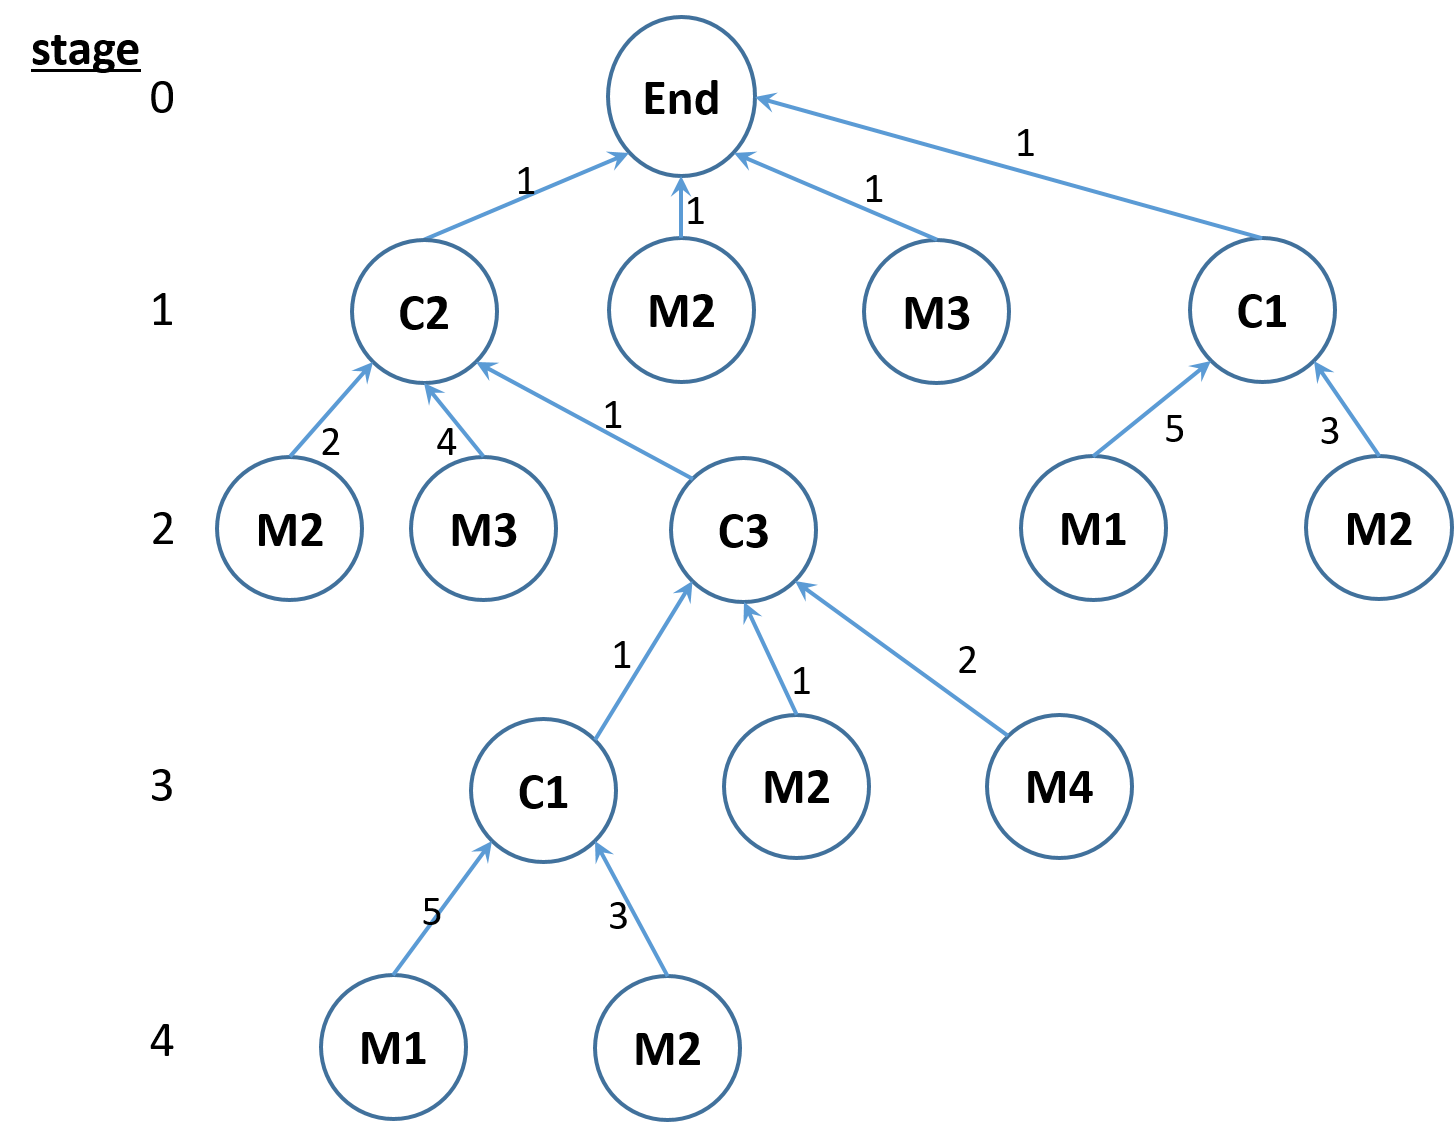
\includegraphics[width=0.49\linewidth]{tree1}
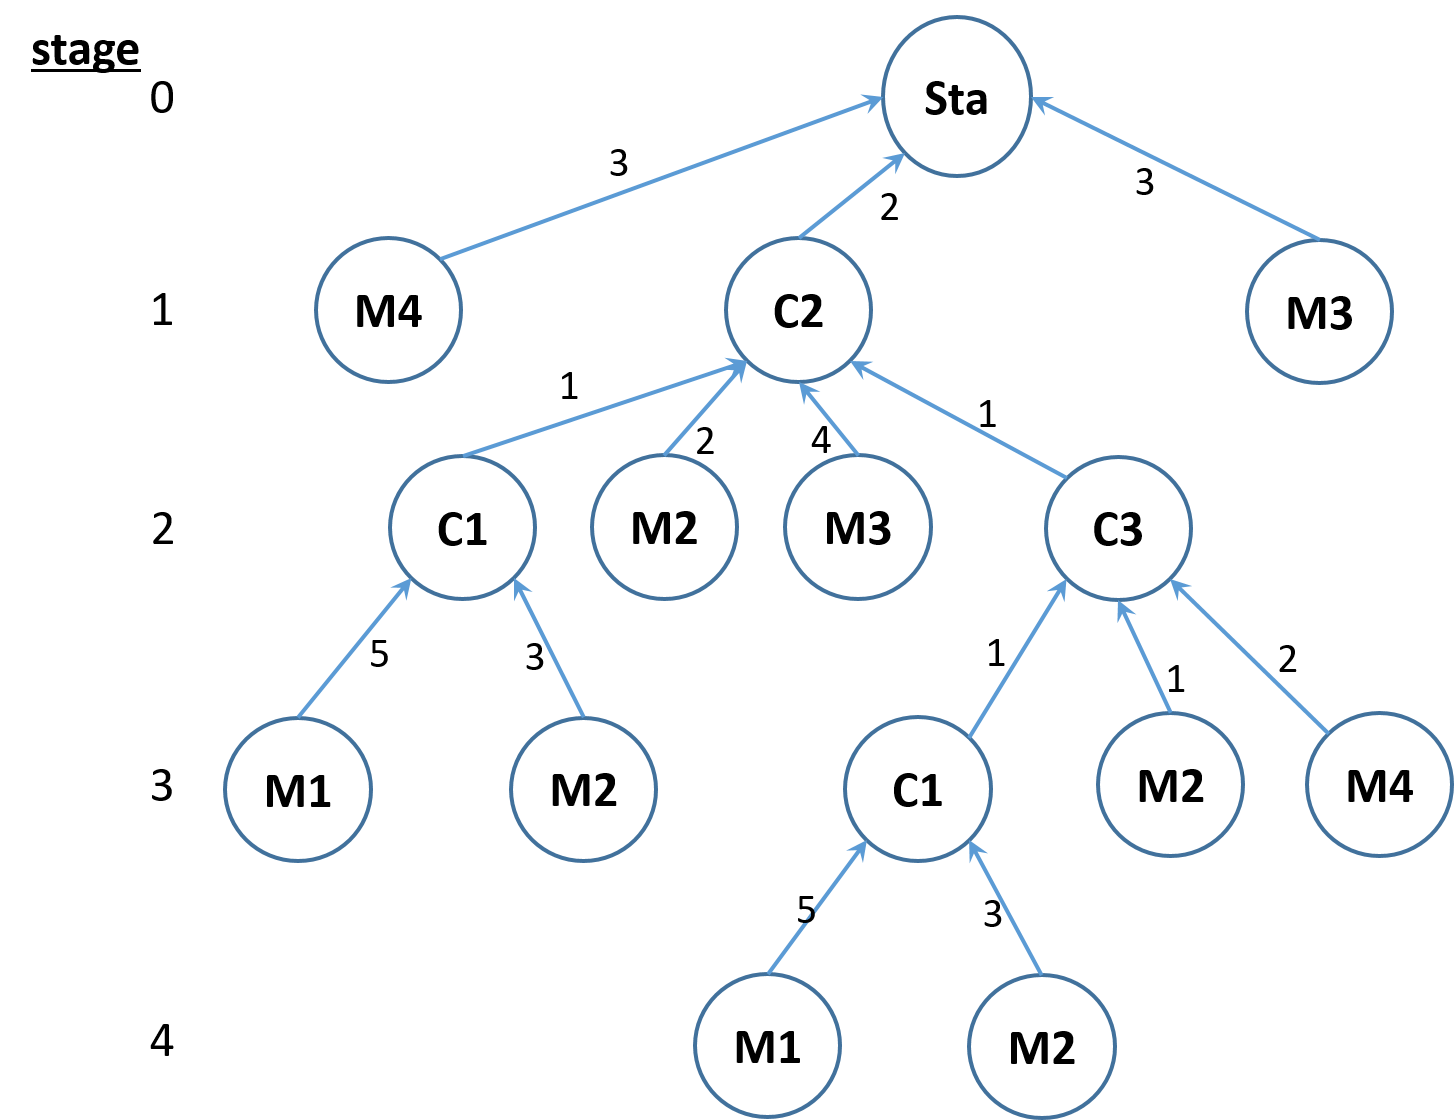
\includegraphics[width=0.49\linewidth]{tree2}

\begin{enumerate}
\def\labelenumi{\arabic{enumi}.}
\setcounter{enumi}{1}
\tightlist
\item
  Deduce the Gozinto graph of the production process and calculate the
  net demand of all materials. (\emph{12 points})
\end{enumerate}

\begin{figure}
\centering
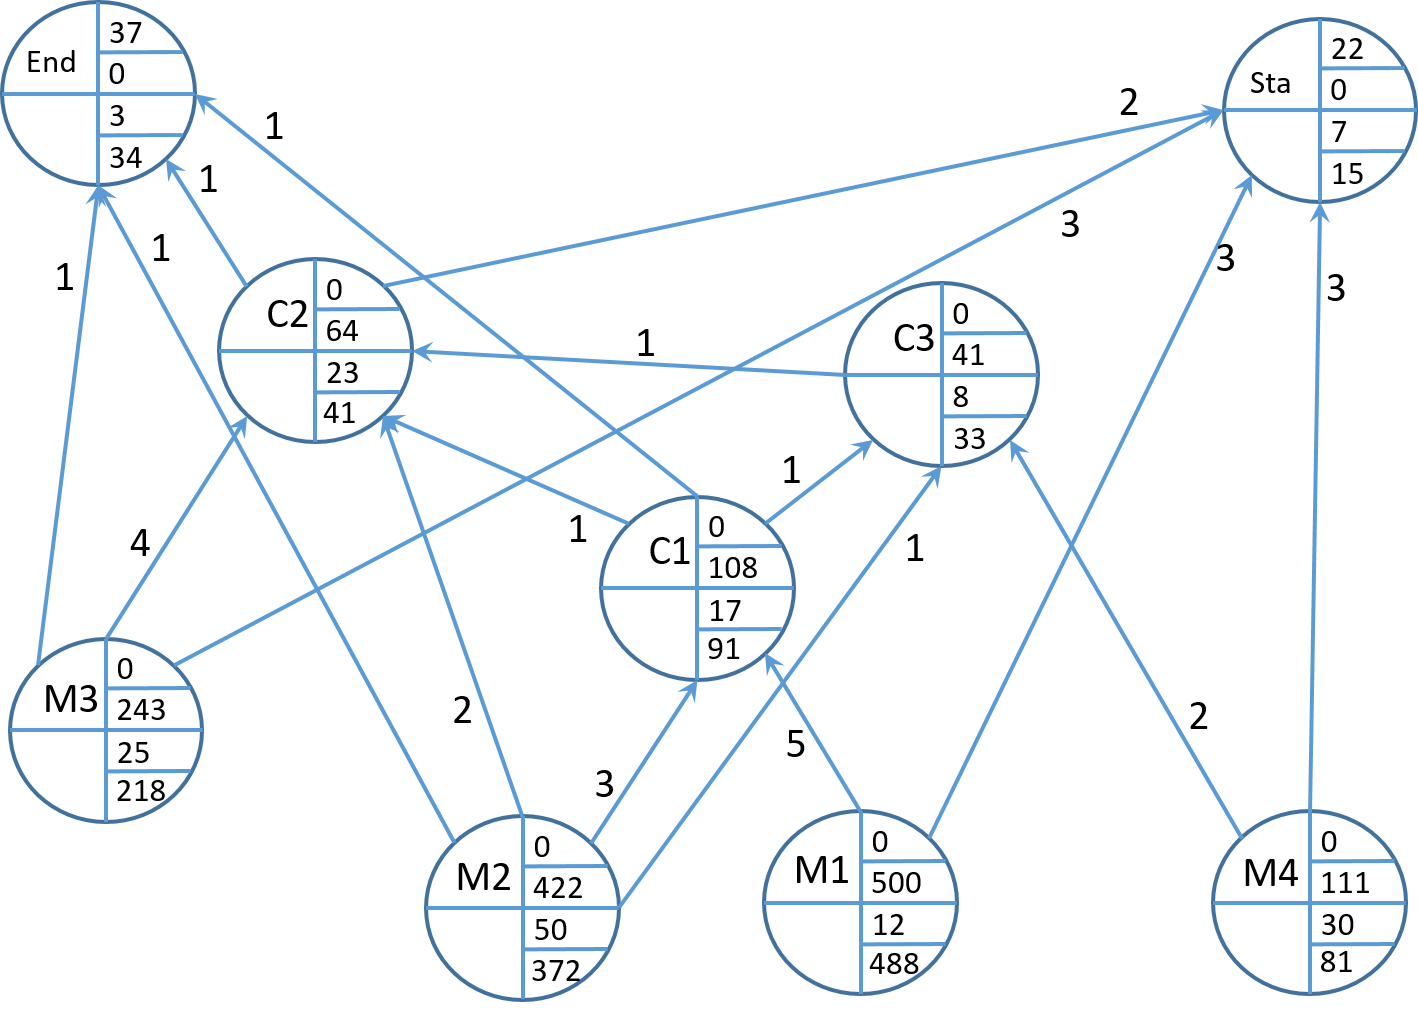
\includegraphics{gozinto.png}
\caption{Gozinto graph}
\end{figure}

\hypertarget{task-2-periodic-review-system}{%
\section{Task 2: Periodic review
system}\label{task-2-periodic-review-system}}

``Leftwing'' intends to provision the most-demand material ``M1'' via
its own warehouse. To control the stocks a periodic review system is to
be established, whereby every week an order is made. The dedicated
supplier promises a lead time of 3 weeks. ``Leftwing'' wants to assure a
stock availability of 98\%. The weekly demand is assumed to be normally
distributed with \(\mu = 400\) and \(\sigma = 100\).

\begin{enumerate}
\def\labelenumi{\arabic{enumi}.}
\tightlist
\item
  Determine the risk period and the distribution of demand in the risk
  period. (\emph{3 points})
\end{enumerate}

The risk period is \(RP = T + L = 1 + 3 = 4\) weeks. Thus, the demand in
the risk period is normally distributed with
\(Y^{RP} \sim N(4 \cdot 400= 1600, 4 \cdot 100^2 )\) (alternatively,
\(\mu^{RP} = 1600\) and \(\sigma^{RP} = 200\))

\begin{enumerate}
\def\labelenumi{\arabic{enumi}.}
\setcounter{enumi}{1}
\tightlist
\item
  Calculate the order-up-to level \(S\) if an \(\alpha\) or a \(\beta\)
  service level of 98\% should be assured (risk period definition).
  (\emph{6 points})
\end{enumerate}

If \(S\) should assure \(\alpha \geq 98\%\), the safety factor is
\(z_{\alpha} \approx 2.0676\) such that
\(S_{\alpha} = \mu_{RP} + z_{\alpha} \cdot \sigma_{RP} = 1600 + 2.0676 \cdot 200 = 2013.52 \approx 2014\)
units.

If \(S\) should assure \(\beta \geq 98\%\), the expected shortfall
should be less than \((1-\beta) \cdot \mu_{RP} = 32\). Thus, the safety
factor \(z_{\beta}\) solves
\(z_{\beta} = L^{-1}\left(Z, \frac{(1-\beta) \cdot \mu_{RP}}{\sigma_{RP}} \right) = L^{-1} (Z,0.16) \approx 0.62\).
Therefore, \(S_{\beta } = 1600 + 0.62 \cdot 200 = 1724\) units.

\begin{enumerate}
\def\labelenumi{\arabic{enumi}.}
\setcounter{enumi}{2}
\tightlist
\item
  A manager of ``Leftwing'' has second thoughts about the supplier. She
  suggests to assume that a lead time of 3 weeks is realized with 60\%
  probability while in 30\% of all cases 4 weeks elapse before the order
  arrives. With 10\% probability the lead time is 5 weeks. Calculate
  \(S\) by approximating the demand in the lead time assuming an
  \(\alpha\) service level of 98\% should be assured. Therefore,
  calculate the expected lead time and lead time variance first.
  (\emph{6 points})
\end{enumerate}

The expectation and variance of the lead time \(L\) are
\(\mu^L = 0.6 \cdot 3 + 0.3 \cdot 4 + 0.1 \cdot 5= 3.5\). The standard
deviation of \(L\) is
\(\sigma^L = \sqrt{0.6 \cdot (3-3.5)^2 + 0.3 \cdot (4-3.5)^2 + 0.1 \cdot (5-3.5)^2} = 0.6708204\).
Thus, for
\(\mu_{RP} = \mu_y \cdot \mu_L + T \cdot \mu_y = 400 \cdot (3.5 + 1 ) = 1800\)
and
\(\sigma_{RP} = \sqrt{\mu_L \cdot \sigma^2_y + \mu^2_y \cdot \sigma_L^2 + T \cdot \sigma_y^2} = \sqrt{3.5\cdot 100^2 + 400^2\cdot 0.6708204^2+ 1\cdot 100^2 } = 342.053\).
Thus, \(S_{\alpha} = 1800 + 2.0676 \cdot 342.053 \approx 2507\) units.

\begin{enumerate}
\def\labelenumi{\arabic{enumi}.}
\setcounter{enumi}{3}
\tightlist
\item
  As the solution of 3. is just an approximation, in which range would
  you expect \(S\) when the lead time distribution is considered
  exactly? (\emph{5 points})
\end{enumerate}

Somewhere between the \(\alpha\)-quantiles when \(L=4\) and L=5\$. I.e.,
\(S^{L=4}_{\alpha} = 5 \cdot 400 + 2.0676 \cdot \sqrt{5} \cdot 100 \approx 2462\)
and
\(S^{L=5}_{\alpha} = 6 \cdot 400 + 2.0676 \cdot \sqrt{6} \cdot 100 \approx 2906\).

Hint: Use the following tabulated values of the standard normal
distribution.

\begin{table}[H]
\centering
\begin{tabular}{r|r|r|>{}r||r|r|r|>{}r||r|r|r|r}
\hline
$z$ & $\varphi(z)$ & $\Phi(z)$ & $L(Z,z)$ & $z$ & $\varphi(z)$ & $\Phi(z)$ & $L(Z,z)$ & $z$ & $\varphi(z)$ & $\Phi(z)$ & $L(Z,z)$\\
\hline
0.0000 & 0.3989 & 0.5000 & 0.3989 & 1.0135 & 0.2387 & 0.8446 & 0.0812 & 2.0270 & 0.0511 & 0.9787 & 0.0079\\
\hline
0.0405 & 0.3986 & 0.5162 & 0.3790 & 1.0541 & 0.2289 & 0.8541 & 0.0751 & 2.0676 & 0.0471 & 0.9807 & 0.0071\\
\hline
0.0811 & 0.3976 & 0.5323 & 0.3597 & 1.0946 & 0.2191 & 0.8632 & 0.0694 & 2.1081 & 0.0432 & 0.9825 & 0.0063\\
\hline
0.1216 & 0.3960 & 0.5484 & 0.3411 & 1.1351 & 0.2095 & 0.8718 & 0.0640 & 2.1486 & 0.0397 & 0.9842 & 0.0056\\
\hline
0.1622 & 0.3937 & 0.5644 & 0.3231 & 1.1757 & 0.1999 & 0.8801 & 0.0590 & 2.1892 & 0.0363 & 0.9857 & 0.0050\\
\hline
0.2027 & 0.3908 & 0.5803 & 0.3058 & 1.2162 & 0.1904 & 0.8880 & 0.0543 & 2.2297 & 0.0332 & 0.9871 & 0.0045\\
\hline
0.2432 & 0.3873 & 0.5961 & 0.2891 & 1.2568 & 0.1811 & 0.8956 & 0.0499 & 2.2703 & 0.0303 & 0.9884 & 0.0040\\
\hline
0.2838 & 0.3832 & 0.6117 & 0.2730 & 1.2973 & 0.1720 & 0.9027 & 0.0458 & 2.3108 & 0.0276 & 0.9896 & 0.0035\\
\hline
0.3243 & 0.3785 & 0.6272 & 0.2576 & 1.3378 & 0.1630 & 0.9095 & 0.0420 & 2.3514 & 0.0251 & 0.9906 & 0.0031\\
\hline
0.3649 & 0.3733 & 0.6424 & 0.2428 & 1.3784 & 0.1543 & 0.9160 & 0.0384 & 2.3919 & 0.0228 & 0.9916 & 0.0028\\
\hline
0.4054 & 0.3675 & 0.6574 & 0.2286 & 1.4189 & 0.1458 & 0.9220 & 0.0352 & 2.4324 & 0.0207 & 0.9925 & 0.0025\\
\hline
0.4459 & 0.3612 & 0.6722 & 0.2150 & 1.4595 & 0.1375 & 0.9278 & 0.0321 & 2.4730 & 0.0187 & 0.9933 & 0.0022\\
\hline
0.4865 & 0.3544 & 0.6867 & 0.2020 & 1.5000 & 0.1295 & 0.9332 & 0.0293 & 2.5135 & 0.0169 & 0.9940 & 0.0019\\
\hline
0.5270 & 0.3472 & 0.7009 & 0.1896 & 1.5405 & 0.1218 & 0.9383 & 0.0267 & 2.5541 & 0.0153 & 0.9947 & 0.0017\\
\hline
0.5676 & 0.3396 & 0.7148 & 0.1777 & 1.5811 & 0.1143 & 0.9431 & 0.0243 & 2.5946 & 0.0138 & 0.9953 & 0.0015\\
\hline
0.6081 & 0.3316 & 0.7284 & 0.1665 & 1.6216 & 0.1071 & 0.9476 & 0.0221 & 2.6351 & 0.0124 & 0.9958 & 0.0013\\
\hline
0.6486 & 0.3233 & 0.7417 & 0.1557 & 1.6622 & 0.1002 & 0.9518 & 0.0200 & 2.6757 & 0.0111 & 0.9963 & 0.0011\\
\hline
0.6892 & 0.3146 & 0.7546 & 0.1455 & 1.7027 & 0.0936 & 0.9557 & 0.0182 & 2.7162 & 0.0100 & 0.9967 & 0.0010\\
\hline
0.7297 & 0.3057 & 0.7672 & 0.1358 & 1.7432 & 0.0873 & 0.9594 & 0.0164 & 2.7568 & 0.0089 & 0.9971 & 0.0009\\
\hline
0.7703 & 0.2965 & 0.7794 & 0.1266 & 1.7838 & 0.0813 & 0.9628 & 0.0149 & 2.7973 & 0.0080 & 0.9974 & 0.0008\\
\hline
0.8108 & 0.2872 & 0.7913 & 0.1179 & 1.8243 & 0.0755 & 0.9659 & 0.0134 & 2.8378 & 0.0071 & 0.9977 & 0.0007\\
\hline
0.8514 & 0.2777 & 0.8027 & 0.1097 & 1.8649 & 0.0701 & 0.9689 & 0.0121 & 2.8784 & 0.0063 & 0.9980 & 0.0006\\
\hline
0.8919 & 0.2680 & 0.8138 & 0.1019 & 1.9054 & 0.0649 & 0.9716 & 0.0109 & 2.9189 & 0.0056 & 0.9982 & 0.0005\\
\hline
0.9324 & 0.2583 & 0.8244 & 0.0946 & 1.9459 & 0.0601 & 0.9742 & 0.0098 & 2.9595 & 0.0050 & 0.9985 & 0.0004\\
\hline
0.9730 & 0.2485 & 0.8347 & 0.0877 & 1.9865 & 0.0555 & 0.9765 & 0.0088 & 3.0000 & 0.0044 & 0.9987 & 0.0004\\
\hline
\end{tabular}
\end{table}

\hypertarget{task-4-joint-economic-lot-sizing}{%
\section{Task 4: Joint Economic Lot
Sizing}\label{task-4-joint-economic-lot-sizing}}

The main component of all drones produced by ``Leftwing'' are the
rotors. In total, ``Leftwing'' manufactures 5 different type of rotors
labeled R1 to R5. All are produced on the same machine. The
production-specific information are summarized as follows:

\begin{longtable}[]{@{}llllll@{}}
\toprule
component & R1 & R2 & R3 & R4 & R5\tabularnewline
\midrule
\endhead
holding cost rate \(c^{sh}_i\) & 0.20 & 0.15 & 0.17 & 0.25 &
0.17\tabularnewline
setup cost \(c^{or}_i\) & 50 & 250 & 185 & 50 & 150\tabularnewline
demand rate \(y_i\) & 25 & 15 & 10 & 30 & 20\tabularnewline
production rate \(p_i\) & 150 & 100 & 90 & 110 & 120\tabularnewline
setup time \(s_i\) & 0.1 & 0.1 & 0.1 & 0.2 & 0.2\tabularnewline
\bottomrule
\end{longtable}

\begin{enumerate}
\def\labelenumi{\arabic{enumi}.}
\tightlist
\item
  Calculate the independent and the common-cycle solution as well as the
  associated total costs. Is the independent solution feasible?
  (\emph{10 points})
\end{enumerate}

The independent solution is given by calculating
\(T_i = \sqrt{\frac{2 \cdot c^{or}_i}{c^{sh}_i \cdot y_i \cdot (1-\rho_i)}}\)
and \(b_i = T_i \cdot \rho_i + s_i\).

\begin{verbatim}
##       [,1]  [,2]  [,3]  [,4]  [,5]
## rho   0.17  0.15  0.11  0.27  0.17
## T     4.90 16.17 15.65  4.28 10.29
## b     0.92  2.53  1.84  1.37  1.91
## cost 20.41 30.92 23.65 23.35 29.15
\end{verbatim}

The total cost of the independent solution is 127.49. The solution is
probably not feasible as the batch time of product does not fit between
subsequent lots of products 1 and 4.

The common cycle solution, first calculates
\(T^{best} = \max(T^*, \underline{T})=\) 9.29 with
\(T^*=\sqrt{\frac{2\cdot \sum c_i^{or}}{\sum c_i^{sh} \cdot y_i \cdot (1-\rho_i)}}=\)
9.29 and \(\underline{T} =\frac{\sum s_i}{1-\sum \rho_i}=\) 5.27.

\begin{verbatim}
##       [,1]  [,2]  [,3]  [,4]  [,5]
## b     1.65  1.49  1.13  2.73  1.75
## cost 24.73 35.80 26.93 30.72 29.31
\end{verbatim}

The total cost of the common-cycle solution is 147.49.

\begin{enumerate}
\def\labelenumi{\arabic{enumi}.}
\setcounter{enumi}{1}
\tightlist
\item
  Calculate the first iteration of the power-of-2 heuristic. Is the
  solution feasible? (\emph{10 points})
\end{enumerate}

First, the basic cycle interval \(B\) is to be determined as
\(B=\min(T_i)\) of the independent solution,i.e., \(B=\) 4.28. Then, the
multiplier \(m_i = \frac{T_i}{B}\) are calculated and rounded the
closest powre of 2.

\begin{verbatim}
##    [,1] [,2] [,3] [,4] [,5]
## m  1.14 3.78 3.65    1  2.4
## m* 1.00 4.00 4.00    1  2.0
\end{verbatim}

Afterwards,\(B\) is reoptimized by
\(B^* = \sqrt{\frac{ 2 \cdot \sum \frac{c_i^{or}}{m_i^*}} {\sum c_i^{sh} \cdot y_i \cdot m_i^* \cdot (1-\rho_i)} } =\)
4.43. Thus, for the batch times \(b_i\) and cycle times \(T_i\) follows

\begin{verbatim}
##   [,1]  [,2]  [,3] [,4] [,5]
## b 0.84  2.76  2.07 1.41 1.68
## T 4.43 17.70 17.70 4.43 8.85
\end{verbatim}

As the idle time in each basic period is just \(4.43-0.84-1.41 = 2.18\),
the solution is not feasible as \(b_2 = 2.76 > 2.18\).

\end{document}
